\documentclass[12pt]{article}
%%%%%%%%%%%%%%%%%%%%%%%%%%%%%%%%%%%%%%%%%%%%%%%%%%%%%%%%%%%%%%%%%%%%%%%%%%%%%%%%%%%%%%%%%%%%%%%%%%%%%%%%%%%%%%%%%%%%%%%%%%%%%%%%%%%%%%%%%%%%%%%%%%%%%%%%%%%%%%%%%%%%%%%%%%%%%%%%%%%%%%%%%%%%%%%%%%%%%%%%%%%%%%%%%%%%%%%%%%%%%%%%%%%%%%%%%%%%%%%%%%%%%%%%%%%%
\usepackage{amsfonts}
\usepackage{eurosym}
\usepackage{geometry}
\usepackage{amsmath,amsthm,amssymb}
\usepackage{graphicx}
\usepackage{comment}
%\usepackage[sort,comma]{natbib}
\usepackage[backend=biber, style = apa]{biblatex}
\usepackage{placeins} % to separate sections

\usepackage{adjustbox}
\usepackage{array}
\usepackage{multirow}
\usepackage{graphicx}
\usepackage{subcaption}
\usepackage{pifont}
\usepackage{amssymb}
\usepackage{comment}
\usepackage[utf8]{inputenc}
\usepackage{setspace}
\usepackage[hang, flushmargin, bottom]{footmisc}
\usepackage{footnotebackref}
\usepackage{xcolor}
\usepackage{hyperref}
\usepackage{booktabs}
\usepackage{pifont}
\usepackage{caption}
\usepackage{float}
\usepackage{todonotes}
\setcounter{MaxMatrixCols}{10}
%TCIDATA{OutputFilter=LATEX.DLL}
%TCIDATA{Version=5.50.0.2960}
%TCIDATA{<META NAME="SaveForMode" CONTENT="1">}
%TCIDATA{BibliographyScheme=BibTeX}
%TCIDATA{LastRevised=Sunday, April 28, 2024 18:12:38}
%TCIDATA{<META NAME="GraphicsSave" CONTENT="32">}
%TCIDATA{Language=American English}

%\setlength{\bibsep}{0.3pt}
\setlength{\textfloatsep}{5pt}
\hypersetup{breaklinks=true,hypertexnames=false,colorlinks=true,citecolor = teal}
\captionsetup{font=normalsize}
\newcommand{\cmark}{\ding{51}}
\def\sym#1{\ifmmode^{#1}\else\(^{#1}\)\fi}
\renewcommand{\thetable}{\Roman{table}}
\geometry{verbose,tmargin=.9in,bmargin=1in,lmargin=1in,rmargin=.9in,nomarginpar}
\makeatletter
\DeclareTextSymbolDefault{\textquotedbl}{T1}
\theoremstyle{plain}
\newtheorem{thm}{\protect\theoremname}
\theoremstyle{plain}
\newtheorem{prop}[thm]{\protect\propositionname}
\providecommand{\propositionname}{Proposition}
\providecommand{\theoremname}{Theorem}
\makeatother
\providecommand{\propositionname}{Proposition}
\providecommand{\theoremname}{Theorem}
\newtheorem{ass}[thm]{Assumption}
% \input{tcilatex}
\usepackage{tikz}
\usetikzlibrary{shapes.geometric, arrows, positioning}





\addbibresource{references.bib}
\begin{document}
 
% \title{{\Large Centralized annuities marketplace}}
%\author{Lucas Condeza\thanks{Yale University %\texttt{lucas.schmitz@yale.edu}}} 
%\date{}
%\maketitle




\subsection*{Institutional Context and Data}\label{sec: context and data}

Chile operates a fully funded, defined-contribution pension system. Throughout their working lives, individuals are required to contribute 10\% of their wages to a personal retirement account. These accounts are managed by private Pension Fund Administrators (PFAs), who invest the funds in a mix of equities, bonds, and mutual funds. Upon reaching retirement age individuals must convert their savings into a stream of retirement income by selecting a pension product. Retirees are generally not allowed to make lump-sum withdrawals.


\textbf{Pension products} 

Retirees opting for a Phased Withdrawal (PW) maintain their savings accounts under PFA management and make systematic withdrawals based on an actuarial formula set by the government.  Under this arrangement, retirees retain ownership of their remaining savings, which can be passed on as an inheritance if they die prematurely. However, they bear the risk of outliving their savings, as pension payments decline over time until the account is depleted. Retirees under PW are also exposed to fluctuations in interest rates, leading to potential volatility in the value of their pension savings.

As an alternative to the Phased Withdrawal, the retiree can purchase an annuity from an insurance company. This choice entails the individual giving up ownership of their savings in exchange for longevity insurance: the insurance company contracts an obligation to pay a fixed, inflation-adjusted amount for the remaining duration of the retiree’s lives. The retiree therefore transfers their longevity risk to the insurance company but gives up the possibility of bequeathing part of their pension savings.

Retirees have the ability to tailor their annuity contracts, particularly by selecting guarantee and deferral options. A guarantee period ensures that the annuity will continue to make payments for a minimum period, offering some protection against early death while still allowing for a potential bequest. Retirees can also allocate a portion of their savings to purchase a deferred annuity, using the remaining balance to increase initial payouts. It is possible to combine guarantee and deferral features within a single contract.

To assist with decision-making, retirees can request and receive multiple quotes through a centralized exchange platform (SCOMP), ultimately choosing among options listed in a document known as the Offers Certificate. The typical retiree requests quotes for around 10 different product types and receives more than 100 quotes overall.
The range of available pension products involves inherent trade-offs among securing higher initial payments, insuring against longevity risk, and preserving wealth for heirs. Thus, selecting the optimal pension product depends critically on how product features interact with an individual's expected lifespan, desire to leave an inheritance, risk tolerance, and degree of impatience. 


\textbf{Centralized exchange}

By regulation, the process that leads to the purchase of an annuity takes place in SCOMP.  Established in 2004, SCOMP was designed to enhance retirees' access to information about their available options and to simplify the process of obtaining and comparing offers from various insurance companies and PFAs (CMF, 2019). Individuals who have accumulated savings above a minimum threshold can request quotes for annuities with different combinations of guarantee and deferral periods. These quote requests are circulated to all insurance companies active in the market, accompanied only by basic information: the retiree’s age, gender, marital status, the age of any legal beneficiaries, and the total amount of savings. Each insurer then decides whether to respond with a quote for each requested pension product.

 
 

 All offers — including Phased Withdrawal offers from PFAs and annuity offers from insurance companies — are compiled into a  document called the Offers Certificate (see figure \ref{fig:offer_ann1}), which is mailed to the retiree. All quotes must be stated in "UF," an inflation-indexed unit of account, ensuring that annuity values are presented in real terms. Retirees also receive information about the risk rating assigned to each insurance company, an important consideration since retirees are only partially protected in the event of insurer insolvency. 
 
Once they receive the Offers Certificate, retirees can either accept one of the offers, postpone their decision, or request an external offer, which is an additional offers from the insurance companies to improve the initial offers. If the retiree is paying an intermediary he will contact the insurers asking for better terms, otherwise the retiree retirees must physically visit the branch of the insurance company. It is important to note that firms are prohibited from offering worse terms during this stage. On average, negotiated offers improve the initial terms modestly, with increases of around 2\% in generosity compared to the original SCOMP offers (\cite{illanes_retirement_2019}).

The number of retirees using SCOMP has increased through time, reaching over 50, 000 in 2018, at which point the annual value of the pension market was over 6 billion dollars . From 2004 onwards, 19 insurance companies have participated in the annuity market. For a majority of them, annuities constitute an important business line, making up over 60\% of both revenues and liabilities. Insurance companies are differentiated by their risk rating, an evaluation of their creditworthiness assessed periodically by two independent agencies. The regulator explicitly forbids the bundling of pension products with other types of insurance. Nevertheless, insurance companies might also differ in terms of their customer service, office locations and brand appeal.

\begin{figure}
    \centering
    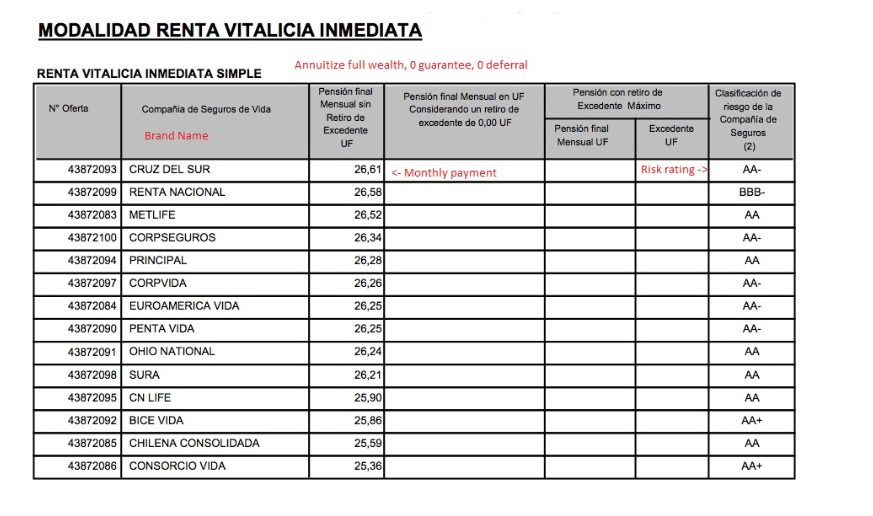
\includegraphics[width=0.85\linewidth]{figures/annuity_offer.png}
    \caption{Annuity offer (source \textcite{illanes_retirement_2019}}
    \label{fig:offer_ann1}
\end{figure}



%%%%%%%%%%%%%%%%%%%%%%%%%%%%%%%%%
%%%%%%%%%%%%%%%%%%%%%%%%%%%%%%%%%
\subsection*{Data}

Centralized offer exchange database SCOMP, available from the regulating agencies, which contains all retirees from August 2004 until July 2020. This database includes basic demographic information about retirees – age, gender, and legal dependents – total savings, geographic location at the city/precinct level. The data also records every offer received by each potential retiree, information about intermediation, pension product accepted, and commission paid. Finally, I also observe the date of death if it occurs before July 2021. I complement this information with publicly available reports on insurance companies’ risk ratings, information about the number of intermediaries, and their registered locations. 



The great advantage of the setting and associated data is that 1. we observe the non-selected offers and 2. the consumer observes all the offers. If the market is not centralized the consumer might not request a quote from every single insurer, whereas here they request one quote and all the insurers bid, and also even when the consumer requests multiple quotes, if the data only includes realized transactions, the quotes will not be observed by the econometrician. 

 


\subsection*{Research questions}

Our research question is: what are the equilibrium impacts of external offers? 


\subsection*{Model}
We model the demand and supply for annuities and how it interacts with the aftermarket. 

\textbf{Demand}
 
Individuals are indexed by $i\in \mathcal{I}$, they are grouped into types depending on their observed characteristics (age, gender, marital status, age of legal beneficiaries and savings decile). Types are indexed by $k \in \mathcal{K}$, with $k(i)$ being the type of individual $i$, insurers are indexed by $j\in \mathcal{J}$.  The utility of $i$ when accepting offer $j$ is: 

\begin{align}\label{eq:utility}
   u_{ijt} = \beta X_{jt}+ \alpha_{k(i)} r_{ij} + \xi_j +\xi_{jt} + \varepsilon_{ijt}   
\end{align}

where $r_{ij}$ is the interest rate, $X_{jt}$  are insurer characteristics (credit-rating, number of customer service offices), $\xi_j$ are persistent unobserved insurer characteristics, and  $\xi_{jt}$ are mean-zero demand shocks.  
The distinctive feature is that the interest rate is at the individual level, for estimation it requires individual level prices. 

Define the mean utility $\delta_{jt} = \beta X_{jt} + \xi_j + \xi_{jt}$, $J_i$ the set of insurers who send an offer to individual $i$ and $Y_i$ the savings of $i$. 

 
Assume that insurers offer a single price for all individuals of a given type,  and the set of insurers making an offer is the same within a type of individuals. In this case, for any individual of type $k$ the probability of buying an annuity from $j$ is: 


\begin{align*}
    s_{kj} = Pr_{kj}((r_{kj})_{j}|\theta, X) = \frac{\exp(\delta_{jt} + \alpha_{k}r_{kj})}{\sum_{j'\in J_k}\exp(\delta_{kt} + \alpha_kr_{ik'})}
\end{align*}


\textbf{Supply model}

In our model insurer differentiation generates market power, we assume that in every other aspect they are homogeneous.


Insurers form beliefs about the remaining years of life of an individual type $k$, denote by $F_k(a)$ the probability they assigned to the individual surviving at least $a$ additional periods. 

Insurer's financing cost is denoted by $\bar{r}_t$, then the profits derived from enrolling an individual $i$ of type $k$ when making an offer $r_{kj}$ are: 

\begin{align}\label{eq:individual_profits}
    \pi_{i}(r_{k(i)j}) = Y_k -   \sum_{t=1}^{\infty} F_{k(i)}(t) \frac{P(r_{k(i)j},Y_k)}{(1+\bar{r}_t)^t} 
\end{align}

where $P(r_{kj})$ is the associated monthly payment with the interest rate offered by the insurer. This monthly payment is constructed using the official mortality tables constructed by the regulator, in what follows we explain their construction. 

The regulator publishes mortality tables based on age and gender, denote by $k^m \in \mathcal{K}^m$ an age-gender combination and by $F_k^m(a)$ the probability that the mortality table assigns to an individual type $k^m$ of living at least $a$ additional years, then $P(r_{kj},Y_k)$ solves:

\begin{align}
    Y_k = \sum_{t=1}^{\infty} F_k^m(t) \frac{P(r_{kj},Y_k)}{(1+r_{kj})^t} 
\end{align}


Then, firms profits in the from types $k$ are given by: 
\begin{align}
    \pi_{jk}( r_k) = \left[Y_k -   \sum_{t=1}^{\infty} F_k(t) \frac{P(r_{kj},Y_k)}{(1+\bar{r}_t)^t} \right] s_{kj}
\end{align}

Assume $F_k(a)$ is generated by their associated $F_k^m(a)$, then the pricing FOC is: 
\begin{align}\label{eq:FOC_simplified}
    - \frac{\partial P(r_{kj},Y_k)}{\partial r_{kj}}  \sum_{t=1}^{\infty}  \frac{F_k^m(t)}{(1+\bar{r}_t)^t}  
    + \left[Y_k -   \sum_{t=1}^{\infty} F_k^m(t) \frac{P(r_{kj},Y_k)}{(1+\bar{r}_t)^t} \right] 
    \alpha_{k}(1-s_{jk}) =0
\end{align}


\textbf{Aftermarket negotiation}






\subsection*{Estimation}
Estimation of the demand model can be done via ML: 
\begin{enumerate}
    \item Estimate  ($\delta_{jt}, \alpha_k$) to maximize the likelihood 
    \item Use $\mathbb{E}[\delta_{jt}|x_{jt},x_{-jt}]= 0$ to estimate ($\beta, \xi_j, \xi_{jt}$)
\end{enumerate}

Moreover, if we assume that firms use the mortality tables published by the regulator to create beliefs over the remaining time, then from equation \ref{eq:FOC_simplified} we can recover the financing costs of the firms. Note that in this case identifying firm-specific financing costs -firm specific $\bar{r}_{jt}$ would be possible. 

The fixed cost is identified from the variation in choosing to apply for external offers. 




\printbibliography
 
\end{document}
